% main.tex -- IEEE conference article (IEEEtran, two-column).
% Build:  cd docs/paper && latexmk -pdf -interaction=nonstopmode main.tex
% Figures: uv run --no-project --with numpy --with pandas --with matplotlib python scripts/make_paper_figures.py
% Every number in this file is taken from a repository file; the source is given in a %-comment next to each
% table/figure and in docs/report/tables/key_numbers.json and docs/paper/figures/paper_figure_numbers.json.
% Placeholders for the author to fill are marked [LIKE THIS] (search for "\placeholder").
\documentclass[conference]{IEEEtran}
\IEEEoverridecommandlockouts
\usepackage[utf8]{inputenc}
\usepackage[T1]{fontenc}
\usepackage{cite}
\usepackage{amsmath,amssymb}
\usepackage{graphicx}
\usepackage{booktabs}
\usepackage{multirow}
\usepackage[table]{xcolor}
\usepackage{microtype}
\usepackage{url}
\usepackage[hidelinks]{hyperref}
\graphicspath{{figures/}}
\newcommand{\placeholder}[1]{\textit{[#1]}}
\newcommand{\pts}{\,pts}
\newcommand{\pmsd}[2]{#1{\scriptsize$\,\pm\,$#2}}
\setlength{\tabcolsep}{4pt}

\begin{document}
\bstctlcite{IEEEexample:BSTcontrol}

\title{Frozen Vision--Language Features Outperform Fine-Tuned CNNs and ViTs for Electronic-Component Recognition
on a Leakage-Audited Web-Scraped Dataset}

\author{\IEEEauthorblockN{Sebastian Klopper}
\IEEEauthorblockA{\placeholder{Department, University}\\
\placeholder{City, Country}\\
\placeholder{email address}}}

\maketitle

\begin{abstract}
Recognising electronic components in internet photographs is a 20-class fine-grained task trained on small, noisy,
web-scraped data. We audit a public Kaggle scrape of 3,530 files. It contains 587 redundant exact copies and 13
conflicting-label duplicate groups, and an automated CLIP screen flags 27.8\% of the retained images as out of scope.
An earlier file-level split leaked duplicates and inflated accuracy by 5.5--13.6 points. Under cluster-grouped
5-fold cross-validation we compare eleven model families, from HOG features and a scratch CNN through ImageNet CNNs
and transformers to DINOv2, CLIP and SigLIP, in zero-shot, linear-probe and fine-tuning regimes. A logistic-regression
probe on frozen SigLIP So400m features reaches macro-F1 $0.824\pm0.012$ with 23k trainable parameters, above every
fine-tuned network (ImageNet fine-tunes: 0.548--0.654). Fine-tuning still beats the probe for ImageNet, DINOv2 and
CLIP-B backbones, but not for SigLIP. The final calibrated, abstaining model scores 83.7\% accuracy (95\% CI
79.9--87.0\%) on a sealed test split evaluated once, and 82.1\% on a separately collected Wikimedia holdout, where its
zero-shot head adds 4.2 points. On the earlier protocol's identical test files it scores 87.7\%, against the
earlier best of 71.3\%.
\end{abstract}

\begin{IEEEkeywords}
image classification, transfer learning, vision--language models, linear probing, data leakage, label noise,
selective classification, electronic components
\end{IEEEkeywords}

% =====================================================================================================================
\section{Introduction}
Electronics hobbyists, teaching laboratories and repair benches handle bins of loose parts: resistors, capacitors,
relays, crystal oscillators, microcontroller boards. A camera-based recogniser that names the part, or admits that it
cannot, is a useful assistant and a natural small-data transfer-learning problem. The classes are visually
fine-grained (a diode and a resistor are both small axial cylinders), and the public training data are web scrapes
whose class names double as everyday English words (\emph{switch}, \emph{transformer}, \emph{fuse}).

Reported accuracies on such data are hard to interpret. Image-search scrapes contain many copies of the same picture,
and a split made at the file level puts copies on both sides~\cite{barz2020cifair,kapoor2023leakage}. Our own first
iteration of this project reported 71--76\% accuracy on a file-level split. As shown below, that split leaked, and the
leakage also compressed the gaps between model families. This paper therefore rebuilds the evaluation from the data up
and asks: (i)~how much does each model family and pretraining source contribute when tuning and evaluation are
leakage-free; (ii)~with ${\sim}$2.5k training images, should a pretrained backbone be frozen or fine-tuned;
(iii)~what does accuracy cost; and (iv)~how well does a deployable, calibrated model do on images it has never seen?

\textbf{Contributions.}
\begin{itemize}
\item A \emph{data audit} of the 20-class Kaggle \emph{electronic-component-recognizer} scrape~\cite{kaggle_dataset}:
exact and near-duplicate clustering, conflicting labels, an out-of-scope screen and a confident-learning label audit.
The audit quantifies how much a file-level split inflates accuracy (5.5--13.6\pts).
\item A \emph{leakage-free benchmark} of eleven model families under three adaptation regimes (zero-shot, frozen
linear probe, fine-tuning). It uses cluster-grouped 5-fold cross-validation, per-fold paired comparisons and a
sealed test split that was read once.
\item The finding that \emph{pretraining source dominates}. Frozen SigLIP features with a 23k-parameter linear head
beat every fine-tuned network, while fine-tuning still helps the weaker ImageNet, DINOv2 and CLIP-B backbones.
\item A \emph{calibrated, abstaining model} exported to ONNX and evaluated on two sealed sets: an in-distribution test
split and an independently collected Wikimedia Commons holdout. We also evaluate it on the original dataset with a
seen/unseen breakdown, and replay the earlier protocol for a like-for-like comparison.
\item Ablations reported \emph{with their null results}: learning-rate-schedule fix, test-time flipping,
training-data cleaning and zero-shot fusion.
\end{itemize}

% =====================================================================================================================
\section{Related Work}
\textbf{Transfer learning and architectures.} Features learned on ImageNet~\cite{russakovsky2015imagenet} transfer
to small target tasks~\cite{yosinski2014transferable}, and architectures that are more accurate on ImageNet tend to
transfer better, both as fixed feature extractors and when fine-tuned~\cite{kornblith2019transfer}. We compare residual
CNNs~\cite{he2016resnet,wightman2021rsb}, EfficientNetV2~\cite{tan2021efficientnetv2},
MobileNetV3~\cite{howard2019mobilenetv3}, ConvNeXt~\cite{liu2022convnext}, the Vision
Transformer~\cite{dosovitskiy2020vit,steiner2022augreg} and Swin~\cite{liu2021swin}, plus a VGG-style
CNN~\cite{simonyan2014vgg,ioffe2015bn} trained from scratch and a HOG~\cite{dalal2005hog} + SVM~\cite{cortes1995svm}
baseline.

\textbf{Self-supervised and vision--language pretraining.} Self-distillation (DINO~\cite{caron2021dino},
DINOv2~\cite{oquab2023dinov2}) learns general features without labels. Contrastive image--text pretraining
(CLIP~\cite{radford2021clip}, ALIGN~\cite{jia2021align}, OpenCLIP~\cite{cherti2023openclip}) adds zero-shot
classification from class-name prompts. SigLIP replaces the softmax contrastive loss with a pairwise sigmoid
loss~\cite{zhai2023siglip}, and SigLIP~2 adds captioning and self-distillation objectives~\cite{tschannen2025siglip2}.

\textbf{Linear probes versus fine-tuning.} Linear probes on frozen features are the standard representation-quality
test~\cite{radford2021clip,oquab2023dinov2}. Fine-tuning can distort pretrained features and underperform out of
distribution~\cite{kumar2022finetuning}. Interpolating fine-tuned and zero-shot weights recovers
robustness~\cite{wortsman2022wiseft}. Our fused probe-plus-zero-shot head is a simpler, output-space relative of
that idea.

\textbf{Leakage, duplicates and label noise.} Near-duplicates between training and test splits inflate benchmark
scores~\cite{barz2020cifair}. Leakage is a common cause of irreproducible ML results~\cite{kapoor2023leakage}, and
networks readily memorise training images~\cite{zhang2017rethinking}. Embedding-based near-duplicate removal is also used to curate
web-scale training data~\cite{abbas2023semdedup}. Grouped (blocked) cross-validation is the remedy for structured
dependence~\cite{roberts2017cv}. Selecting a model on the same folds that score it biases the
estimate~\cite{varma2006bias}, and freshly collected test sets can reveal accuracy drops that the original test set
hides~\cite{recht2019imagenet}.
Confident learning finds label errors from out-of-sample probabilities~\cite{northcutt2021confident}, and such
errors are pervasive even in test sets~\cite{northcutt2021pervasive}.

\textbf{Calibration and selective classification.} Modern networks are miscalibrated, and temperature scaling is a
strong fix~\cite{guo2017calibration}. Rejecting low-confidence inputs trades coverage for
accuracy~\cite{chow1970reject,geifman2017selective}; the maximum softmax probability is the usual confidence
score~\cite{hendrycks2017baseline}.

\textbf{Electronic-component recognition.} Much of the vision work on electronics targets
printed-circuit-board inspection under controlled imaging~\cite{ling2023pcb}. For classification of loose components, Shao~\emph{et~al.} compare twelve
fine-tuned ImageNet models and report 92.26--99.95\% accuracy~\cite{shao2025electronic}. Zhou and Zhang propose a CNN
for components on diverse backgrounds~\cite{zhou2025electronic}. Their data and splits differ from ours, so the
numbers are not comparable. Our audit shows why the split construction must be reported alongside any such
accuracy.

% =====================================================================================================================
\section{Dataset and Audit}\label{sec:data}
\textbf{Source.} The images come from the Kaggle \emph{electronic-component-recognizer}
dataset~\cite{kaggle_dataset}, a web scrape with 20 class folders: battery holder, breadboard, capacitor, connector,
crystal oscillator, diode, fuse, heat sink, IC chip, inductor coil, jumper wire, LED, microcontroller board,
potentiometer, power supply module, relay, resistor, switch, transformer and transistor. The formats are mixed: among
the 2,943 unique decoded files there are 1,486 JPEG, 787 WebP, 402 PNG, 245 AVIF, 20 GIF and 3 MPO images, and 345
needed alpha compositing. A build script decodes every file, collapses exact duplicates by SHA-256, links
near-duplicates and writes a versioned manifest with one row per unique image (Table~\ref{tab:audit}).

% SOURCE: data/v2/leakage_report.json (counts); docs/report/tables/data_audit.csv
\begin{table}[t]
\centering\footnotesize
\caption{Data-cleaning pipeline. Near-duplicate and out-of-scope rows are flags on retained rows, not removals.}
\label{tab:audit}
\begin{tabular}{@{}lr@{}}
\toprule
Stage & Images \\
\midrule
Raw image files & 3,530 \\
Unique files (SHA-256) & 2,943 \\
Rows kept (conflicting-label exact duplicates removed) & 2,930 \\
Duplicate clusters (grouping unit for every split) & 2,787 \\
Rows in near-duplicate clusters & 234 \\
Rows flagged out-of-scope (automated CLIP screen) & 816 \\
\bottomrule
\end{tabular}
\end{table}

\textbf{Exact duplicates and conflicting labels.} The 3,530 raw files contain only 2,943 unique images: 533
duplicate groups hold 587 redundant copies. Thirteen exact-duplicate groups carry two different labels (e.g.\ the
same picture under \emph{fuse} and \emph{relay}). All 13 groups were excluded, leaving 2,930 rows.

\textbf{Near-duplicates.} Perceptual hashing (pHash radius 10) combined with CLIP cosine similarity ($\geq$0.85 with
a pHash match, $\geq$0.92 without) links 234 rows into 91 near-duplicate clusters of size 2--29. Two of these
clusters mix labels; their 4 rows are kept and flagged. With the singletons there are 2,787 clusters.

\textbf{Out-of-scope content.} A CLIP zero-shot screen scores each image against the 20 class prompts and nine
distractor concepts (person, car, food, logo, text screenshot, cartoon/game art, circuit schematic, website
screenshot, collage). It flags an image when the distractor probability mass exceeds 0.25. It flags 816 rows
(27.8\%; 704 dev, 112 test). The most frequent top distractors are circuit schematics (245), logos (180),
cartoon/game art (130) and people (83). Contamination concentrates in classes named by common words
(Fig.~\ref{fig:ood}). 121 of 177 \emph{switch} images are flagged, mostly Nintendo Switch consoles and game art, as
are 64 of 128 \emph{transformer} images (toy robots, cartoons). The screen is automated and was not human-verified;
some flags, e.g.\ resistor schematics, are arguably in scope.

% SOURCE: data/v2/manifest.json (flags) via scripts/make_paper_figures.py -> figures/paper_figure_numbers.json
\begin{figure}[t]
\centering
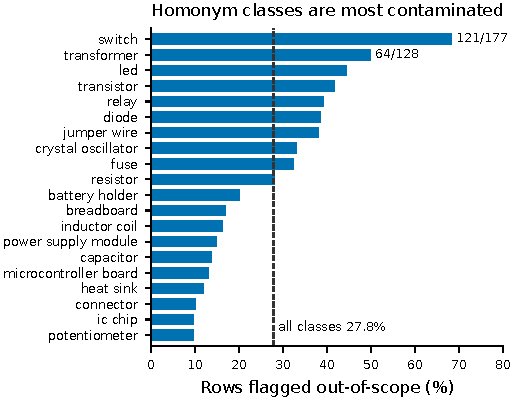
\includegraphics[width=\columnwidth]{fig1_ood_per_class}
\caption{Share of each class flagged out-of-scope by the automated CLIP distractor screen (threshold 0.25; $n$ = 2,930
rows). Dashed line: all classes. Numbers give flagged/total for the two worst classes.}
\label{fig:ood}
\end{figure}

\textbf{Label errors.} A confident-learning-style audit~\cite{northcutt2021confident} on out-of-fold probe
probabilities lists 69 confident label issues, 11 of which are also out-of-scope flags. The most common patterns are
diode$\to$transistor, microcontroller board$\to$IC chip and jumper wire$\to$breadboard (4 each).

\textbf{Decision.} Flagged rows were \emph{kept} for training and evaluation. We report all-row scores and
\emph{in-scope} scores over rows without the out-of-scope flag. Section~\ref{sec:ablations} shows that removing the
flagged rows from training hurts.

% =====================================================================================================================
\section{Evaluation Protocol}\label{sec:protocol}
\textbf{Splits.} Whole duplicate clusters are assigned to splits (seed 42), so copies and near-copies of an image never
sit on both sides of any split~\cite{roberts2017cv}. A sealed \emph{test} split of 418 rows (16--25 per class) is held
out first. The remaining 2,512 \emph{dev} rows form five cluster-grouped folds. The largest total-variation distance
between class distributions across the outer grouped split is 0.017. All model selection used dev folds only. The test
split is readable only through an explicit confirmation flag. It was read \emph{once}, for the final model, after
every design choice had been frozen. A second sealed set, the web holdout (Section~\ref{sec:gen}), was collected after
the final model was frozen.

\textbf{Metrics.} The primary metric is macro-F1 over the 20 classes. Accuracy is secondary. Cross-validated scores are
mean\,$\pm$\,SD over the five folds. In-scope accuracy is pooled over folds. Test accuracies carry 95\% Wilson
intervals~\cite{wilson1927}. With 418 test images the binomial standard error is $\pm$1.8 points, so test-split
differences below about 3.5 points are not resolvable. Calibration is measured by the expected calibration error (ECE,
15 equal-width bins)~\cite{guo2017calibration}. Selective prediction is summarised as coverage (fraction answered)
and accepted accuracy (accuracy on answered images)~\cite{geifman2017selective}.

\textbf{Why the earlier split leaked.} The first iteration of the project split \emph{files}, not clusters (a
70/15/15 split). Of the 853 images in its validation and test splits, 198 (23.2\%) duplicate a training image.
Table~\ref{tab:leak} replays three linear probes under both protocols. On the duplicated rows the probes are nearly
perfect (95--99\%). The legacy-style score is inflated by 5.5 points for SigLIP and by 11.0 and 13.6 points for
ConvNeXt-T and ResNet-50: weaker models gain most, because memorised copies stand in for the features they lack. The
inflation therefore also \emph{compresses} the gaps between families. Accuracy on the non-duplicated legacy rows is
still above grouped-CV accuracy (e.g.\ 0.860 vs.\ 0.825 for SigLIP). Near-duplicates missed by the exact-duplicate
count and differences between the evaluation sets are the likely causes; we do not decompose this residual further.

% SOURCE: results/leakage_simulation.csv ; docs/report/tables/leakage_simulation.csv
% NOTE: produced by analysis code not in the repository (see Section X, provenance).
\begin{table}[t]
\centering\footnotesize
\caption{Leakage simulation: accuracy of linear probes under grouped CV and under the legacy file-level split (853
evaluation rows, 198 of them duplicates of a training image).}
\label{tab:leak}
\begin{tabular}{@{}lrrrrr@{}}
\toprule
Probe backbone & \shortstack{Grouped\\CV} & \shortstack{Legacy\\split} & \shortstack{Infl.\\(pts)} &
\shortstack{Dup.\\rows} & \shortstack{Other\\rows} \\
\midrule
ResNet-50 & 0.5215 & 0.6577 & +13.6 & 0.9949 & 0.5557 \\
ConvNeXt-T & 0.5983 & 0.7081 & +11.0 & 0.9646 & 0.6305 \\
SigLIP So400m & 0.8252 & 0.8804 & +5.5 & 0.9495 & 0.8595 \\
\bottomrule
\end{tabular}
\end{table}

% =====================================================================================================================
\section{Models and Adaptation Regimes}\label{sec:models}
Table~\ref{tab:taxonomy} lists the families, grouped by \emph{pretraining source}, which turns out to be the main axis
of variation. Pretrained weights come from \texttt{timm}~\cite{wightman2021rsb} and
\texttt{open\_clip}~\cite{cherti2023openclip}.

% SOURCE: docs/report/REPORT.md Table 3 (src/compclass/models/registry.py); params from results/benchmark.csv
\begin{table}[t]
\centering\footnotesize
\caption{Model families. IN = ImageNet. Parameter counts are the trainable parameters of the fine-tuning runs;
(B): ViT-B variant; SigLIP So400m has 428.2M.}
\label{tab:taxonomy}
\begin{tabular}{@{}l@{\hspace{4pt}}l@{\hspace{3pt}}r@{}}
\toprule
Family (variants) & Pretraining & \shortstack{Params\\(M)} \\
\midrule
HOG + HSV hist.\ + SVM~\cite{dalal2005hog,cortes1995svm} & none (hand-crafted) & -- \\
VGG-style CNN~\cite{simonyan2014vgg,ioffe2015bn} & none (from scratch) & 1.2 \\
ResNet-50~\cite{he2016resnet,wightman2021rsb} & IN-1k & 23.5 \\
EfficientNetV2-S~\cite{tan2021efficientnetv2} & IN-21k$\to$1k & 20.2 \\
MobileNetV3-L~\cite{howard2019mobilenetv3} & IN-1k & 4.2 \\
ConvNeXt-T~\cite{liu2022convnext} & IN-22k$\to$1k & 27.8 \\
ViT-B/16~\cite{dosovitskiy2020vit,steiner2022augreg} & IN-21k$\to$1k & 85.8 \\
Swin-T~\cite{liu2021swin} & IN-22k$\to$1k & 27.5 \\
DINOv2 ViT-S/B/L-14~\cite{oquab2023dinov2} & LVD-142M, self-distill. & 85.7\,(B) \\
CLIP ViT-B/16, L/14(@336)~\cite{radford2021clip} & 400M image--text pairs & 85.8\,(B) \\
SigLIP, SigLIP~2 B/16, So400m~\cite{zhai2023siglip,tschannen2025siglip2} & WebLI image--text & 92.9\,(B) \\
\bottomrule
\end{tabular}
\end{table}

\textbf{Zero-shot} (vision--language models only): each image is assigned to the class whose template-averaged text
embedding (``a photo of a \{class\}.'', \dots) has the highest cosine similarity. No training images are used.
\textbf{Linear probe}: the backbone is frozen. Features of the evaluation-preprocessed image feed a standardised
logistic regression whose $C$ is chosen inside each training fold by grouped CV. The head has $20(D+1)$ parameters,
about 23k for $D=1152$.
\textbf{Fine-tune}: the pretrained network gets a new head and is trained with one hand-set recipe per family: AdamW
\cite{loshchilov2019adamw}, linear warm-up then cosine decay~\cite{loshchilov2017sgdr}, label smoothing
0.1~\cite{szegedy2016inception}, RandAugment~\cite{cubuk2020randaugment} and fp16 mixed precision. Where configured,
the recipe adds layer-wise learning-rate decay and frozen-backbone warm-up epochs. Early stopping uses fold-validation
macro-F1. SigLIP So400m (428.2M parameters) is too large to fine-tune fully on an 8\,GB GPU, so only its last four
blocks are trained (\emph{partial fine-tune}, 76.2M trainable parameters, folds 0--2 only).
\textbf{Classical}: HOG + HSV colour-histogram features with an RBF-SVM.
All training ran on one NVIDIA RTX 4060 Ti (8\,GB).

% =====================================================================================================================
\section{Results}\label{sec:results}
\subsection{Main benchmark}
Table~\ref{tab:bench} lists the headline rows and Fig.~\ref{fig:bench} shows every backbone and regime.

% SOURCE: results/benchmark.csv (schedule in {-, fixed}); asserted equal to per-fold means of
%   results/phase1/raw/runs.jsonl, results/phase1b/runs.jsonl, results/phase2/runs_fixed.jsonl (max diff 4.9e-5)
%   by scripts/make_report_figures.py. MobileNetV3-L macro-F1 = 0.54754 (per-fold mean) -> 0.548.
\begin{table}[t]
\centering\footnotesize
\caption{Headline results, grouped 5-fold CV over 2,512 dev images (mean\,$\pm$\,SD over folds). ZS = zero-shot,
LP = linear probe, FT = fine-tune. $^\dagger$Partial fine-tune, folds 0--2.}
\label{tab:bench}
\begin{tabular}{@{}llccc@{}}
\toprule
Backbone & Reg. & Macro-F1 & Acc. & In-scope \\
\midrule
SigLIP So400m/14@384 & LP & \pmsd{\textbf{0.824}}{0.012} & 0.825 & 0.861 \\
SigLIP 2 So400m/14@384 & LP & \pmsd{0.814}{0.011} & 0.815 & 0.852 \\
SigLIP So400m/14@384$^\dagger$ & FT & \pmsd{0.812}{0.023} & 0.813 & 0.835 \\
SigLIP So400m/14@384 & ZS & \pmsd{0.776}{0.018} & 0.775 & 0.827 \\
SigLIP 2 B/16 & LP & \pmsd{0.758}{0.014} & 0.760 & 0.792 \\
SigLIP 2 B/16 & FT & \pmsd{0.733}{0.027} & 0.735 & 0.767 \\
CLIP ViT-L/14@336 & LP & \pmsd{0.721}{0.019} & 0.727 & 0.753 \\
CLIP ViT-B/16 & FT & \pmsd{0.702}{0.017} & 0.707 & 0.724 \\
DINOv2 ViT-B/14 & FT & \pmsd{0.668}{0.024} & 0.672 & 0.717 \\
DINOv2 ViT-L/14 & LP & \pmsd{0.667}{0.020} & 0.668 & 0.721 \\
ViT-B/16 (IN-21k) & FT & \pmsd{0.654}{0.032} & 0.659 & 0.712 \\
ConvNeXt-T & FT & \pmsd{0.641}{0.034} & 0.647 & 0.689 \\
Swin-T & FT & \pmsd{0.639}{0.034} & 0.644 & 0.694 \\
EfficientNetV2-S & FT & \pmsd{0.608}{0.024} & 0.616 & 0.653 \\
ResNet-50 & FT & \pmsd{0.580}{0.012} & 0.585 & 0.618 \\
MobileNetV3-L & FT & \pmsd{0.548}{0.016} & 0.556 & 0.584 \\
Scratch CNN & FT & \pmsd{0.355}{0.015} & 0.365 & 0.379 \\
HOG + HSV + SVM & -- & \pmsd{0.206}{0.017} & 0.220 & -- \\
\bottomrule
\end{tabular}
\end{table}

% SOURCE: results/benchmark.csv via scripts/make_paper_figures.py (fig_benchmark); TTA rows omitted
\begin{figure}[t]
\centering
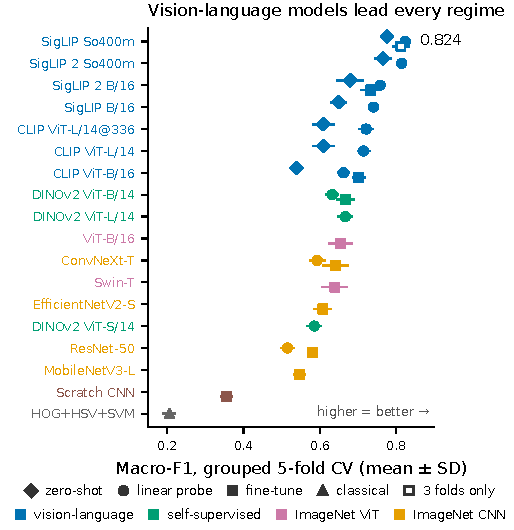
\includegraphics[width=\columnwidth]{fig2_benchmark}
\caption{Macro-F1 of every backbone under each adaptation regime (grouped 5-fold CV, $n$ = 2,512 dev images; bars:
SD over folds). Label colour encodes the pretraining source. The open square (SigLIP So400m partial fine-tune) was run
on folds 0--2 only. All fine-tunes use the fixed learning-rate schedule.}
\label{fig:bench}
\end{figure}

\textbf{Web-scale vision--language pretraining dominates.} The best entries are all SigLIP / SigLIP~2 So400m variants.
Zero-shot SigLIP So400m (0.776), which uses no training images, beats every fine-tuned network except the partial
fine-tune of the same backbone. CLIP ViT-L/14 probes reach 0.715--0.721. Self-supervised DINOv2 is clearly weaker as
a frozen feature (ViT-L 0.667, ViT-B 0.633). Among ImageNet-pretrained networks the transformers (ViT-B 0.654,
Swin-T 0.639) and ConvNeXt-T (0.641) lead; ResNet-50 (0.580) and MobileNetV3-L (0.548) trail. Pretraining \emph{data}
matters more than architecture. Four ViT-B models with 86--93M parameters span 8 points: ViT-B/16 with ImageNet-21k
weights (0.654), DINOv2 ViT-B/14 (0.668), CLIP ViT-B/16 (0.702) and SigLIP~2 B/16 (0.733), all fine-tuned.

\textbf{Learned features are indispensable.} The scratch CNN (0.355) and HOG + SVM (0.206) are far below every
pretrained model. The 19--30-point gap from the scratch CNN to the ImageNet fine-tunes measures what pretraining buys
at this data size.

\textbf{Out-of-scope rows cost every family.} In-scope accuracy exceeds all-row accuracy for every method, by 1.3--5.7
points (0.861 vs.\ 0.825 for the best probe). Part of the remaining error comes from the contaminated data rather
than from the classifier.

\subsection{Frozen probe versus fine-tuning}
Table~\ref{tab:pvf} and Fig.~\ref{fig:pvf} pair each fine-tune with the frozen probe of the same backbone on identical
folds. The answer depends on the backbone. Fine-tuning SigLIP~2 B/16 \emph{loses} 2.5 points to its own probe (0/5
folds better). The SigLIP So400m partial fine-tune loses 0.9 points (1/3 folds), within fold noise. For CLIP ViT-B/16,
DINOv2 ViT-B/14, ConvNeXt-T and ResNet-50, fine-tuning gains 3.6--6.5 points and wins on 5/5 folds. The ``frozen
$\geq$ fine-tuned'' result therefore holds for SigLIP only. Even the best fine-tune of any family (SigLIP So400m
partial, 0.812) does not beat the frozen probe of the same backbone (0.822 on the same folds). This pattern is consistent with
reports that fine-tuning can distort strong pretrained features~\cite{kumar2022finetuning}. One caveat runs against the
probes: fine-tunes early-stop on the fold they are scored on, which biases their CV scores
upward~\cite{varma2006bias}. The SigLIP result is therefore conservative.

% SOURCE: docs/report/tables/probe_vs_finetune.csv (per-fold records results/phase1/raw/runs.jsonl,
%   results/phase2/runs_fixed.jsonl); figures/paper_figure_numbers.json key probe_vs_ft
\begin{table}[t]
\centering\footnotesize
\caption{Paired probe vs.\ fine-tune macro-F1 on identical folds. $\Delta$ = fine-tune $-$ probe.}
\label{tab:pvf}
\begin{tabular}{@{}lcccrc@{}}
\toprule
Backbone & Folds & Probe & Fine-tune & $\Delta$ (pts) & FT wins \\
\midrule
SigLIP 2 B/16 (full) & 0--4 & 0.758 & 0.733 & $-$2.52 & 0/5 \\
SigLIP So400m (partial) & 0--2 & 0.822 & 0.812 & $-$0.92 & 1/3 \\
DINOv2 ViT-B/14 & 0--4 & 0.633 & 0.668 & +3.57 & 5/5 \\
CLIP ViT-B/16 & 0--4 & 0.662 & 0.702 & +3.99 & 5/5 \\
ConvNeXt-T & 0--4 & 0.593 & 0.641 & +4.78 & 5/5 \\
ResNet-50 & 0--4 & 0.515 & 0.580 & +6.52 & 5/5 \\
\bottomrule
\end{tabular}
\end{table}

% SOURCE: per-fold records as Table V, via scripts/make_paper_figures.py (fig_probe_vs_ft)
\begin{figure}[t]
\centering
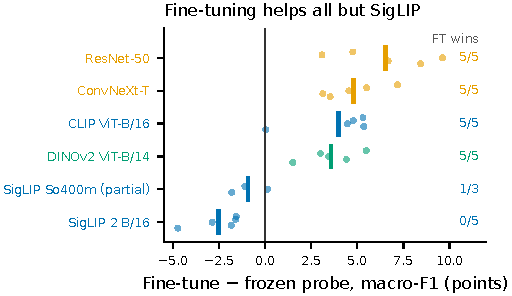
\includegraphics[width=\columnwidth]{fig3_probe_vs_finetune}
\caption{Per-fold macro-F1 gain of fine-tuning over the frozen linear probe of the same backbone (dots: folds; bars:
means; right: folds where fine-tuning wins). SigLIP So400m uses the partial fine-tune on folds 0--2.}
\label{fig:pvf}
\end{figure}

\subsection{Accuracy versus cost}
Among fine-tunes, accuracy follows the pretraining source rather than compute. MobileNetV3-L trains in 0.7\,min per
fold and ResNet-50 in 1.6\,min. The SigLIP So400m partial fine-tune needs 17.5\,min (76.2M trainable parameters,
3.8\,GB peak VRAM) and still does not beat its probe. On the trainable-parameter axis the Pareto front consists almost
entirely of linear probes (Fig.~\ref{fig:cost}). A 23k-parameter logistic regression on frozen SigLIP So400m features
matches or exceeds a 76M-parameter fine-tune. The relevant deployment cost is therefore the inference cost of the
frozen backbone (Section~\ref{sec:final}), not training.

% SOURCE: results/benchmark.csv (+ feature dims from results/phase1/raw/runs.jsonl) via make_paper_figures.py
\begin{figure}[t]
\centering
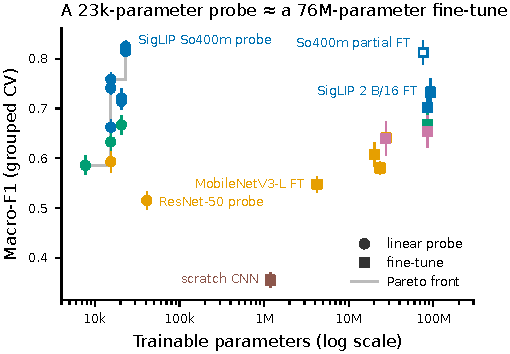
\includegraphics[width=\columnwidth]{fig4_params}
\caption{Macro-F1 vs.\ trainable parameters for fine-tunes and linear probes (probe = $20(D+1)$ weights; zero-shot
models have none and are omitted). Colours as in Fig.~\ref{fig:bench}; bars: SD over folds; open square: 3 folds.
Grey: Pareto front.}
\label{fig:cost}
\end{figure}

% =====================================================================================================================
\section{Ablations}\label{sec:ablations}
Table~\ref{tab:abl} summarises the ablations. Most of the effects lie inside the noise floor of this data size.

% SOURCE: docs/report/tables/ablations.csv (results/phase1b/runs.jsonl vs results/phase1/raw/runs.jsonl;
%   results/phase1/cleaning_ablation_siglip_so400m.csv; exports/final/fit_report.json; results/final/final_test_v2.json;
%   results/benchmark.csv); schedule: results/schedule_ablation_folds012.csv, key_numbers.json schedule_*
\begin{table}[t]
\centering\footnotesize
\caption{Ablations on the SigLIP So400m model (MF1 = macro-F1, Acc = accuracy, IS = in-scope accuracy).}
\label{tab:abl}
\begin{tabular}{@{}llrrr@{}}
\toprule
Ablation & Metric & Base & Variant & $\Delta$ (pts) \\
\midrule
hflip TTA, SigLIP So400m probe & MF1 & 0.824 & 0.819 & $-$0.50 \\
hflip TTA, SigLIP 2 So400m probe & MF1 & 0.814 & 0.820 & +0.57 \\
drop 69 label issues (train) & IS & 0.861 & 0.863 & +0.16 \\
drop OOD-flagged rows (train) & IS & 0.861 & 0.852 & $-$0.89 \\
zero-shot fusion, dev OOF & Acc & 0.825 & 0.826 & +0.16 \\
zero-shot fusion, sealed test & Acc & 0.845 & 0.837 & $-$0.72 \\
zero-shot fusion, web holdout & Acc & 0.779 & 0.821 & +4.18 \\
partial FT, 137M, old schedule & MF1 & 0.822 & 0.821 & $-$0.10 \\
partial FT, 76M, fixed schedule & MF1 & 0.822 & 0.812 & $-$0.92 \\
\bottomrule
\end{tabular}
\end{table}

\textbf{Partial fine-tuning.} Two partial fine-tunes of SigLIP So400m were run on folds 0--2: 137.2M trainable
parameters with the old schedule (0.821, 23.3\,min/fold) and the last four blocks, 76.2M parameters, with the fixed
schedule (0.812, 17.5\,min/fold). The probe scores 0.822 on the same folds. Neither beats it, so the final model keeps
the backbone frozen.

\textbf{Learning-rate schedule fix (null result).} The first fine-tuning runs did not restart the warm-up when the
backbone unfroze. The fix also froze BatchNorm statistics during the head-only phase. Evaluated on folds 0--2 for ten
families, it improved 14 of 30 fold scores, with a mean change of +0.19 points (exact two-sided sign test $p=0.86$).
The SD of the per-fold differences is 1.4 points, a $\pm$1.6-point noise floor (2\,SE) for a 3-fold mean. Only the
BatchNorm CNNs moved consistently upward: ResNet-50 (+2.0, 3/3 folds), EfficientNetV2-S (+1.6, 2/3) and
MobileNetV3-L (+0.8, 3/3). This points to the BatchNorm change rather than the warm-up, but the two are confounded.

\textbf{Test-time flipping} changed probe macro-F1 by $-$0.50 (SigLIP, 1/5 folds better) and +0.57 points
(SigLIP~2, 5/5 folds better). The effect is inconsistent and below one point, so TTA, which doubles inference cost,
was not adopted.

\textbf{Training-data cleaning hurts.} Dropping the 69 audited label issues from training changed in-scope accuracy
by +0.16 points, which is noise. Dropping all out-of-scope-flagged rows \emph{reduced} in-scope accuracy by 0.9 points
and all-row accuracy by 3.3 points (0.825$\to$0.792). Many flagged rows evidently still carry class signal, or
resemble the flagged evaluation images. The training data were left unchanged.

\textbf{Zero-shot fusion.} The final model adds the backbone's zero-shot log-probabilities to the probe's,
$\log p_\text{probe} + 0.25\log\operatorname{softmax}(50\cos)$, with weight and temperature fixed a priori. In
distribution this is a null result: +0.16 points out-of-fold and $-$0.72 points on the sealed test, a tie within
the $\pm$1.8-point standard error. Per-image probe-only test predictions were not saved, so no paired (McNemar) test is
possible. Fusion was kept because it is free at inference (one extra $1152\times20$ product). On the out-of-source
web holdout it adds 4.2 points (Section~\ref{sec:gen}).

% =====================================================================================================================
\section{Final Model and Deployment}\label{sec:final}
\textbf{Model.} The final model is the frozen SigLIP So400m/14 image tower at 384\,px. Its 1152-d feature feeds
(i)~a standardised logistic-regression probe ($C=0.01$) refit on all 2,512 dev rows and (ii)~the zero-shot text head,
fused as above. Preprocessing resizes the short side to 427 (bicubic), centre-crops to 384 and normalises with
mean = std = 0.5. A temperature $T=0.8977$, fit on dev out-of-fold fused scores, lowers out-of-fold ECE from 0.050 to
0.029~\cite{guo2017calibration}. The model abstains when its maximum probability is below 0.5. This is the smallest
grid threshold whose out-of-fold accepted accuracy is at least 0.90 (coverage 0.846 at 0.909 accepted accuracy).

\textbf{Sealed test (evaluated once).} The model scores accuracy 0.837 (95\% CI 0.799--0.870) and macro-F1 0.834 on
the 418 sealed test images (Table~\ref{tab:sealed}), within one standard error of its dev out-of-fold estimate
(0.826). There is thus no sign of selection overfitting. In-scope accuracy is 0.869 ($n=306$); the 112
out-of-scope-flagged rows score 0.750. Errors are spread over many class pairs, and no off-diagonal confusion cell
exceeds 2 images. The clear weakness is \emph{resistor} recall: 0.545 (12/22, precision 1.00), with the ten misses
scattered over seven classes. Power supply module (F1 0.711) and capacitor (0.788) come next. The high \emph{switch}
score (recall 0.96) is partly an artefact. 19 of the 25 test switch images are out-of-scope flagged (mostly Nintendo
Switch material), and 18 of those 19 are predicted correctly: the test split shares the scrape's contamination.

% SOURCE: results/final/final_test_v2.json (+_preds.npz), results/final/final_test_web_holdout_v1.json,
%   exports/final/fit_report.json (dev OOF); Wilson CIs in figures/paper_figure_numbers.json
\begin{table}[t]
\centering\footnotesize
\caption{Final model on the two sealed sets, each evaluated once.}
\label{tab:sealed}
\begin{tabular}{@{}lcc@{}}
\toprule
Metric & \shortstack{Kaggle sealed\\test ($n=418$)} & \shortstack{Web holdout\\($n=407$)} \\
\midrule
Accuracy & 0.837 & 0.821 \\
\quad 95\% Wilson CI & 0.799--0.870 & 0.780--0.855 \\
Macro-F1 & 0.834 & 0.816 \\
Probe-only accuracy (no zero-shot head) & 0.845 & 0.779 \\
Coverage at threshold 0.5 & 0.871 & 0.853 \\
Accuracy on accepted images & 0.909 & 0.891 \\
ECE (15 bins) & 0.034 & 0.050 \\
\bottomrule
\end{tabular}
\end{table}

\textbf{Calibration and abstention.} After temperature scaling the model is well calibrated on unseen data (test ECE
0.034; Fig.~\ref{fig:calib}a). Abstention behaves on the test split much as it did out-of-fold: at threshold 0.5 the
model answers 87.1\% of test images (out-of-fold 84.6\%) and is right on 90.9\% of them (out-of-fold 90.9\%).
Raising the threshold to 0.8 answers 70.8\% of test images at 97.0\% accuracy.

% SOURCE: results/final/final_test_v2_preds.npz (asserted equal to final_test_v2.json), exports/final/fit_report.json
\begin{figure}[t]
\centering
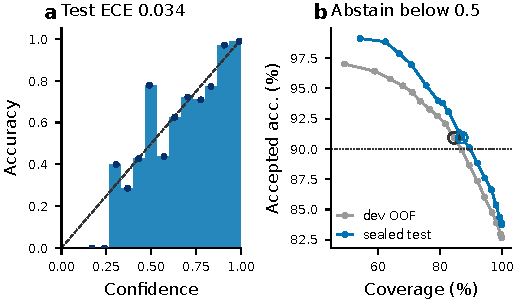
\includegraphics[width=\columnwidth]{fig5_calibration_abstention}
\caption{(a) Reliability diagram on the sealed test ($n=418$; 15 bins; bar = accuracy, dot = mean confidence; bins with
few images are noisy). (b) Coverage vs.\ accuracy on answered images when abstaining below a confidence threshold
(0--0.95, step 0.05) for dev out-of-fold scores ($n$ = 2,512) and the sealed test. Circles: chosen threshold 0.5;
dotted: 90\% target.}
\label{fig:calib}
\end{figure}

\textbf{Export and latency.} The image tower and both heads are exported as one ONNX graph (1,637\,MB, external-data
format) with \texttt{logits} and \texttt{probs} outputs. In onnxruntime it matches PyTorch to a maximum absolute
probability difference of $6.3\times10^{-6}$ with 100\% argmax agreement. Batch-1 latency is 892\,ms per image on
the CPU execution provider and 67\,ms with the CUDA provider (16-core desktop CPU, RTX 4060 Ti). OpenCV's DNN importer
cannot load the graph (\texttt{readNetFromONNX} terminates with a segmentation fault). The demonstrators therefore
use onnxruntime for inference. A Python/OpenCV application classifies files, folders, URLs or webcam frames and draws
the top-3 labels or \emph{UNSURE}; its webcam and window modes have not yet been tested on a display.
Its predictions match the PyTorch reference on 64 dev images (maximum
$|\Delta p| = 9.1\times10^{-6}$). A Rust/GPUI desktop front end using onnxruntime is under development.

% =====================================================================================================================
\section{Generalisation Beyond the Test Split}\label{sec:gen}
Fig.~\ref{fig:gen} collects three further checks of the frozen final model.

% SOURCE: results/final/final_test_v2.json; results/final/final_test_web_holdout_v1.json;
%   results/kaggle_original/summary.json (by_v2_split, legacy_test_replay; old best from legacy/docs/EXPERIMENT_LOG.md)
\begin{figure}[t]
\centering
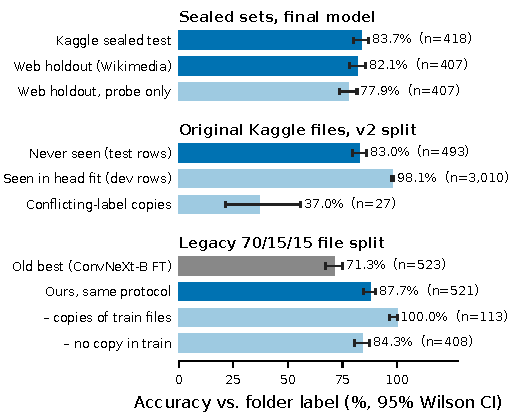
\includegraphics[width=\columnwidth]{fig6_generalisation}
\caption{Accuracy of the final model against the folder label with 95\% Wilson intervals. Top: the two sealed sets.
Middle: all 3,530 original Kaggle files grouped by the v2 split of their image (dev rows were used to fit the
head). Bottom: the earlier 70/15/15 file-level protocol, with our probe refit on legacy-train rows only, against the
earlier best fine-tune on the same test files.}
\label{fig:gen}
\end{figure}

\textbf{Out-of-source web holdout.} A second sealed set of 407 Wikimedia Commons photographs (CC/PD licensed, 15--25
per class) was built after the model was frozen. Construction comprised category listing, exact deduplication, and
a CLIP ViT-B/32 leakage gate against every training-pool image (cosine $\geq$0.92 dropped; maximum kept similarity
0.903). The nine photos already shown in the demo were excluded, and a strict visual review kept only photos in which
one component of the labelled class is dominant. Evaluated once, the model reaches accuracy 0.821 (95\% CI
0.780--0.855) and macro-F1 0.816 (Table~\ref{tab:sealed}), close to its in-distribution accuracy. Here the zero-shot
head pays off. The fused model is correct on 334 images versus 317 for the probe alone (+4.2 points), in line with
evidence that retaining a vision--language model's zero-shot classifier preserves robustness to distribution
shift~\cite{wortsman2022wiseft}. The weakest classes mirror the training contamination: \emph{LED} recall 0.47 (7
errors predicted \emph{diode}), \emph{switch} 0.52 (real toggle, slide and DIP switches predicted \emph{IC chip} 6
times, since the training \emph{switch} class is dominated by game consoles) and \emph{transformer} 0.67 (5 errors to
\emph{inductor coil}).

\textbf{All original Kaggle files.} Scored on all 3,530 original files, the model reaches 95.5\%. This figure is
misleading, because most files are copies of rows used to fit the head (98.1\% on 3,010 such files). On the 493 files
whose image lies in the sealed test split, which the model has never seen, accuracy is 83.0\% (86.5\% on the 348
in-scope ones). The 27 files of conflicting-label duplicate groups score 37.0\%: copies of one image carry
different folder labels, so they cannot all be right. The legacy test files illustrate the trap. As deployed, the model scores 96.6\% on the 523
legacy-test files, but only 71 of them belong to v2 sealed-test rows, and on those it scores 85.9\%.

\textbf{Like-for-like replay of the earlier protocol.} To compare with the first iteration on its own terms, we refit
the probe only on rows containing a legacy-training file (2,129 rows, $C=0.1$). We keep the same backbone and
zero-shot head and score the legacy-test files. The replay reaches 87.7\% ($n=521$; two conflicting-label files not
scored), against 71.3\% for the earlier best (a ConvNeXt-B fine-tune) on the same protocol: +16.4 points. Leaked copies
of training files score 100\% ($n=113$), and the 408 files with no training copy score 84.3\%. The comparison is not
fully independent: the backbone and fusion head were chosen on v2 dev folds, which contain many legacy-test images.
It nevertheless shows that the gain is not an artefact of the stricter protocol.

% =====================================================================================================================
\section{Limitations and Threats to Validity}\label{sec:limits}
\textbf{One source dataset.} All training, CV and sealed-test images come from one Kaggle scrape with shared
search-engine biases. The web holdout tests other internet photographs, but bench photographs from a real camera
remain untested.

\textbf{Automated screens.} The 27.8\% out-of-scope estimate and every in-scope number rest on an unverified CLIP screen
with a hand-set threshold. It has false positives (e.g.\ resistor schematics) and certainly misses some cases. The 69
label issues are likewise model-flagged and unreviewed.

\textbf{Web-holdout construction.} One automated reviewer, looking at thumbnails without a second annotator, kept only
clear single-component photos. The holdout is therefore easier than an unbiased web sample. Five classes have only 15
images, and 144 of 984 selected candidates were never downloaded because of rate limits.

\textbf{Sample size and seeds.} The test standard error is $\pm$1.8 points, and per-class recall rests on 16--25
images. Every configuration was run once per fold with a single seed, so fold SDs (1.0--3.5 points) mix data and
optimisation noise.

\textbf{Unequal tuning.} Fine-tunes used one hand-set recipe per family without a per-family search. Probes tuned $C$
by inner grouped CV, and zero-shot used fixed templates. A per-family search could narrow the probe--fine-tune gap for
some backbones. The So400m partial fine-tune ran on 3 folds only.

\textbf{Confounds and selection bias.} The schedule fix is confounded with BatchNorm freezing. Fine-tunes early-stop
on their scoring fold. The zero-shot fusion weight was suggested by an exploratory dev analysis before being fixed.

\textbf{Deployment.} OpenCV's DNN module cannot run the exported graph, and CPU latency (0.9\,s) is too slow for smooth
webcam use.

\textbf{Provenance.} The benchmark table was cross-checked against the per-fold run records (maximum difference
$4.9\times10^{-5}$). The leakage simulation, schedule ablation and cleaning ablation summaries were produced by
analysis code that is not in the repository; their inputs are.

% =====================================================================================================================
\section{Conclusion and Future Work}\label{sec:conclusion}
On a small, noisy web-scraped component dataset, the choice of pretraining source outweighs architecture, model size
and training compute. A linear probe on frozen SigLIP features beats every fine-tuned CNN and ViT, but fine-tuning is
still the better choice for weaker backbones. The data audit matters as much as the model: file-level splits of the
scrape leak duplicates, inflate accuracy and compress family differences. Reported component-recognition accuracies
should come with a description of how duplicates were handled. The final model meets its 80--85\% target on two
sealed sets and abstains usefully.
Future work: (i)~distil the model~\cite{hinton2015distilling} into a small CNN that OpenCV's DNN module can load and
that runs in real time on a CPU; (ii)~collect and label target-domain camera photographs; (iii)~human relabelling of
the 69 label issues and review of the 816 out-of-scope flags, which would make the in-scope subset a verified
benchmark; (iv)~per-family hyper-parameter search with nested CV and several seeds; and (v)~resistor-specific cues
such as colour-band reading and higher input resolution.

\section*{Acknowledgment}
\placeholder{Acknowledgments, e.g.\ supervisor and funding, to be added by the author.} Code, data manifests and
results: \placeholder{repository URL}.

% IEEEtran bibliography style control: list up to 6 authors, then "et al."
\IEEEtriggeratref{34}
\bibliographystyle{IEEEtran}
\bibliography{refs}

\end{document}
